% Options for packages loaded elsewhere
\PassOptionsToPackage{unicode}{hyperref}
\PassOptionsToPackage{hyphens}{url}
%
\documentclass[
]{article}
\usepackage{amsmath,amssymb}
\usepackage{lmodern}
\usepackage{ifxetex,ifluatex}
\ifnum 0\ifxetex 1\fi\ifluatex 1\fi=0 % if pdftex
  \usepackage[T1]{fontenc}
  \usepackage[utf8]{inputenc}
  \usepackage{textcomp} % provide euro and other symbols
\else % if luatex or xetex
  \usepackage{unicode-math}
  \defaultfontfeatures{Scale=MatchLowercase}
  \defaultfontfeatures[\rmfamily]{Ligatures=TeX,Scale=1}
\fi
% Use upquote if available, for straight quotes in verbatim environments
\IfFileExists{upquote.sty}{\usepackage{upquote}}{}
\IfFileExists{microtype.sty}{% use microtype if available
  \usepackage[]{microtype}
  \UseMicrotypeSet[protrusion]{basicmath} % disable protrusion for tt fonts
}{}
\makeatletter
\@ifundefined{KOMAClassName}{% if non-KOMA class
  \IfFileExists{parskip.sty}{%
    \usepackage{parskip}
  }{% else
    \setlength{\parindent}{0pt}
    \setlength{\parskip}{6pt plus 2pt minus 1pt}}
}{% if KOMA class
  \KOMAoptions{parskip=half}}
\makeatother
\usepackage{xcolor}
\IfFileExists{xurl.sty}{\usepackage{xurl}}{} % add URL line breaks if available
\IfFileExists{bookmark.sty}{\usepackage{bookmark}}{\usepackage{hyperref}}
\hypersetup{
  pdftitle={Evolutionary Rates \& Selection Strength},
  hidelinks,
  pdfcreator={LaTeX via pandoc}}
\urlstyle{same} % disable monospaced font for URLs
\usepackage[margin=1in]{geometry}
\usepackage{color}
\usepackage{fancyvrb}
\newcommand{\VerbBar}{|}
\newcommand{\VERB}{\Verb[commandchars=\\\{\}]}
\DefineVerbatimEnvironment{Highlighting}{Verbatim}{commandchars=\\\{\}}
% Add ',fontsize=\small' for more characters per line
\usepackage{framed}
\definecolor{shadecolor}{RGB}{248,248,248}
\newenvironment{Shaded}{\begin{snugshade}}{\end{snugshade}}
\newcommand{\AlertTok}[1]{\textcolor[rgb]{0.94,0.16,0.16}{#1}}
\newcommand{\AnnotationTok}[1]{\textcolor[rgb]{0.56,0.35,0.01}{\textbf{\textit{#1}}}}
\newcommand{\AttributeTok}[1]{\textcolor[rgb]{0.77,0.63,0.00}{#1}}
\newcommand{\BaseNTok}[1]{\textcolor[rgb]{0.00,0.00,0.81}{#1}}
\newcommand{\BuiltInTok}[1]{#1}
\newcommand{\CharTok}[1]{\textcolor[rgb]{0.31,0.60,0.02}{#1}}
\newcommand{\CommentTok}[1]{\textcolor[rgb]{0.56,0.35,0.01}{\textit{#1}}}
\newcommand{\CommentVarTok}[1]{\textcolor[rgb]{0.56,0.35,0.01}{\textbf{\textit{#1}}}}
\newcommand{\ConstantTok}[1]{\textcolor[rgb]{0.00,0.00,0.00}{#1}}
\newcommand{\ControlFlowTok}[1]{\textcolor[rgb]{0.13,0.29,0.53}{\textbf{#1}}}
\newcommand{\DataTypeTok}[1]{\textcolor[rgb]{0.13,0.29,0.53}{#1}}
\newcommand{\DecValTok}[1]{\textcolor[rgb]{0.00,0.00,0.81}{#1}}
\newcommand{\DocumentationTok}[1]{\textcolor[rgb]{0.56,0.35,0.01}{\textbf{\textit{#1}}}}
\newcommand{\ErrorTok}[1]{\textcolor[rgb]{0.64,0.00,0.00}{\textbf{#1}}}
\newcommand{\ExtensionTok}[1]{#1}
\newcommand{\FloatTok}[1]{\textcolor[rgb]{0.00,0.00,0.81}{#1}}
\newcommand{\FunctionTok}[1]{\textcolor[rgb]{0.00,0.00,0.00}{#1}}
\newcommand{\ImportTok}[1]{#1}
\newcommand{\InformationTok}[1]{\textcolor[rgb]{0.56,0.35,0.01}{\textbf{\textit{#1}}}}
\newcommand{\KeywordTok}[1]{\textcolor[rgb]{0.13,0.29,0.53}{\textbf{#1}}}
\newcommand{\NormalTok}[1]{#1}
\newcommand{\OperatorTok}[1]{\textcolor[rgb]{0.81,0.36,0.00}{\textbf{#1}}}
\newcommand{\OtherTok}[1]{\textcolor[rgb]{0.56,0.35,0.01}{#1}}
\newcommand{\PreprocessorTok}[1]{\textcolor[rgb]{0.56,0.35,0.01}{\textit{#1}}}
\newcommand{\RegionMarkerTok}[1]{#1}
\newcommand{\SpecialCharTok}[1]{\textcolor[rgb]{0.00,0.00,0.00}{#1}}
\newcommand{\SpecialStringTok}[1]{\textcolor[rgb]{0.31,0.60,0.02}{#1}}
\newcommand{\StringTok}[1]{\textcolor[rgb]{0.31,0.60,0.02}{#1}}
\newcommand{\VariableTok}[1]{\textcolor[rgb]{0.00,0.00,0.00}{#1}}
\newcommand{\VerbatimStringTok}[1]{\textcolor[rgb]{0.31,0.60,0.02}{#1}}
\newcommand{\WarningTok}[1]{\textcolor[rgb]{0.56,0.35,0.01}{\textbf{\textit{#1}}}}
\usepackage{graphicx}
\makeatletter
\def\maxwidth{\ifdim\Gin@nat@width>\linewidth\linewidth\else\Gin@nat@width\fi}
\def\maxheight{\ifdim\Gin@nat@height>\textheight\textheight\else\Gin@nat@height\fi}
\makeatother
% Scale images if necessary, so that they will not overflow the page
% margins by default, and it is still possible to overwrite the defaults
% using explicit options in \includegraphics[width, height, ...]{}
\setkeys{Gin}{width=\maxwidth,height=\maxheight,keepaspectratio}
% Set default figure placement to htbp
\makeatletter
\def\fps@figure{htbp}
\makeatother
\setlength{\emergencystretch}{3em} % prevent overfull lines
\providecommand{\tightlist}{%
  \setlength{\itemsep}{0pt}\setlength{\parskip}{0pt}}
\setcounter{secnumdepth}{-\maxdimen} % remove section numbering
\usepackage{booktabs}
\usepackage{longtable}
\usepackage{array}
\usepackage{multirow}
\usepackage{wrapfig}
\usepackage{float}
\usepackage{colortbl}
\usepackage{pdflscape}
\usepackage{tabu}
\usepackage{threeparttable}
\usepackage{threeparttablex}
\usepackage[normalem]{ulem}
\usepackage{makecell}
\usepackage{xcolor}
\ifluatex
  \usepackage{selnolig}  % disable illegal ligatures
\fi

\title{Evolutionary Rates \& Selection Strength}
\author{}
\date{\vspace{-2.5em}}

\begin{document}
\maketitle

This vignette explains how to extract evolutionary rate parameters
estimated from relaxed clock Bayesian inference analyses produced by the
program Mr.~Bayes. It also shows how to use evolutionary rate based
inference of selection strength (or mode) adapted to clock-based rates,
as introduced by
\href{https://www.nature.com/articles/s41559-021-01532-x}{Simões \&
Pierce 2021}.

\hypertarget{evolutionary-rates-statistics-and-plots}{%
\section{Evolutionary Rates Statistics and
Plots}\label{evolutionary-rates-statistics-and-plots}}

Open the \emph{EvoPhylo} package

\begin{Shaded}
\begin{Highlighting}[]
\FunctionTok{library}\NormalTok{(EvoPhylo)}
\CommentTok{\#library(ggplot2)}
\CommentTok{\#library(ggtree)}
\end{Highlighting}
\end{Shaded}

Extract evolutionary rate summary statistics from each node from a
Bayesian clock (time-calibrate) summary tree produced by Mr.~Bayes,
store them in a data frame, produce summary tables, and plots:

\begin{enumerate}
\def\labelenumi{\arabic{enumi}.}
\tightlist
\item
  First, get rates from tree file and create rate table.
\item
  Export the rate table
\end{enumerate}

\begin{Shaded}
\begin{Highlighting}[]
\CommentTok{\#Import summary tree produced by Mr. Bayes}
\NormalTok{tree}\OtherTok{\textless{}{-}}\NormalTok{treeio}\SpecialCharTok{::}\FunctionTok{read.mrbayes}\NormalTok{(}\StringTok{"Tree\_3p.t"}\NormalTok{)}

\CommentTok{\#Get table of clock rates with summary stats for each node in the tree for each relaxed clock partition }
\NormalTok{RateTable\_Medians\_no\_clades }\OtherTok{\textless{}{-}} \FunctionTok{get\_clockrate\_table}\NormalTok{(tree, }\AttributeTok{summary =} \StringTok{"median"}\NormalTok{)}
\NormalTok{RateTable\_Means\_no\_clades }\OtherTok{\textless{}{-}} \FunctionTok{get\_clockrate\_table}\NormalTok{(tree, }\AttributeTok{summary =} \StringTok{"mean"}\NormalTok{)}

\CommentTok{\#Export the rate table}
\CommentTok{\#write.csv(RateTable\_Medians\_no\_clades, file="RateTable\_Medians.csv")}
\CommentTok{\#write.csv(RateTable\_Means\_no\_clades, file="RateTable\_Means.csv")}
\end{Highlighting}
\end{Shaded}

\begin{enumerate}
\def\labelenumi{\arabic{enumi}.}
\setcounter{enumi}{2}
\tightlist
\item
  Import rate table with customized clade membership added as an extra
  column
\item
  Get summary statistics table and plots for each clade by clock
\end{enumerate}

\begin{Shaded}
\begin{Highlighting}[]
\CommentTok{\#Import rate table with clade membership }
\NormalTok{RateTable\_Medians}\OtherTok{\textless{}{-}} \FunctionTok{read.csv}\NormalTok{(}\StringTok{"RateTable\_Medians\_Clades.csv"}\NormalTok{, }\AttributeTok{header =} \ConstantTok{TRUE}\NormalTok{)}

\CommentTok{\#Get summary statistics table for each clade by clock }
\FunctionTok{clockrate\_summary}\NormalTok{(RateTable\_Medians, }\StringTok{"Sum\_RateTable\_Medians.csv"}\NormalTok{, }\AttributeTok{digits=}\DecValTok{2}\NormalTok{)}
\end{Highlighting}
\end{Shaded}

\begin{verbatim}
##                clade clock  n mean   sd  min   Q1 median   Q3  max
## 1        Dipnomorpha     1  8 1.08 0.10 0.93 1.01   1.07 1.16 1.19
## 2     Elpisostegalia     1 14 1.58 0.22 1.11 1.41   1.65 1.78 1.80
## 3     Osteolepididae     1 11 0.60 0.25 0.15 0.43   0.77 0.79 0.84
## 4      Rhizodontidae     1 14 0.54 0.30 0.01 0.31   0.64 0.80 0.85
## 5  Tristichopteridae     1 21 0.69 0.03 0.59 0.67   0.69 0.70 0.75
## 6              Other     1 11 0.87 0.36 0.52 0.68   0.77 0.94 1.79
## 7        Dipnomorpha     2  8 0.72 0.21 0.45 0.58   0.73 0.89 0.98
## 8     Elpisostegalia     2 14 1.31 0.09 1.00 1.31   1.32 1.37 1.38
## 9     Osteolepididae     2 11 0.32 0.15 0.05 0.25   0.35 0.42 0.50
## 10     Rhizodontidae     2 14 0.30 0.18 0.01 0.15   0.35 0.42 0.53
## 11 Tristichopteridae     2 21 0.31 0.06 0.24 0.29   0.29 0.31 0.53
## 12             Other     2 11 0.73 0.25 0.37 0.59   0.69 0.77 1.30
## 13       Dipnomorpha     3  8 0.85 0.12 0.69 0.77   0.87 0.95 0.99
## 14    Elpisostegalia     3 14 0.80 0.15 0.60 0.65   0.85 0.94 0.95
## 15    Osteolepididae     3 11 0.28 0.13 0.06 0.23   0.26 0.39 0.48
## 16     Rhizodontidae     3 14 0.29 0.17 0.01 0.17   0.35 0.40 0.49
## 17 Tristichopteridae     3 21 0.49 0.10 0.32 0.39   0.51 0.57 0.62
## 18             Other     3 11 0.72 0.16 0.45 0.63   0.69 0.80 1.00
\end{verbatim}

Plot distributions of rates by clock partition and clade

\begin{Shaded}
\begin{Highlighting}[]
\CommentTok{\#Overlapping plots}
\FunctionTok{clockrate\_dens\_plot}\NormalTok{(RateTable\_Medians, }\AttributeTok{stack =} \ConstantTok{FALSE}\NormalTok{, }\AttributeTok{nrow =} \DecValTok{1}\NormalTok{, }\AttributeTok{scales =} \StringTok{"fixed"}\NormalTok{)}
\end{Highlighting}
\end{Shaded}

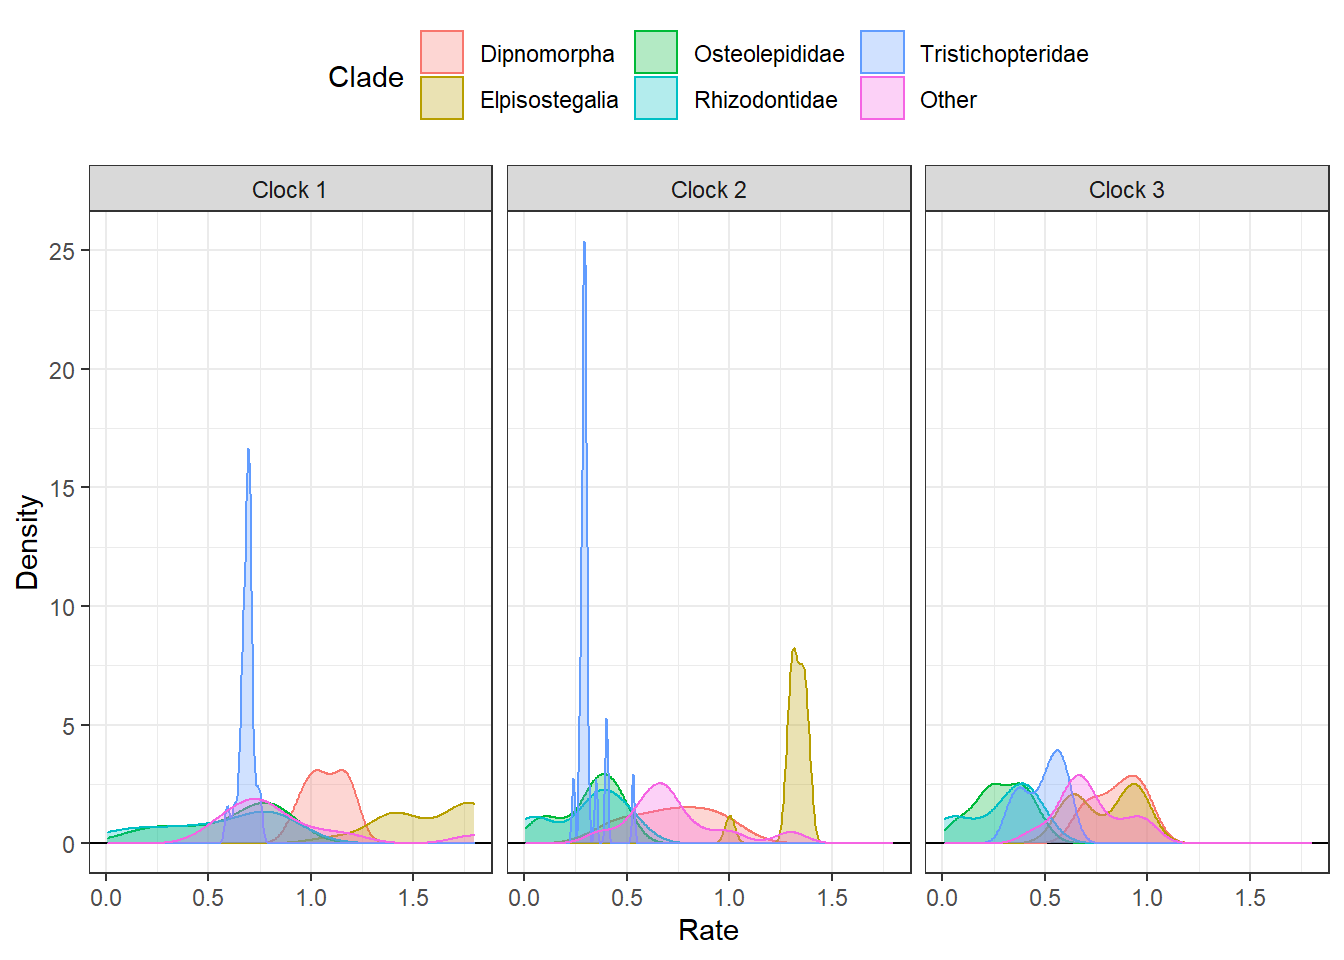
\includegraphics{Vignette-Tetrapod_files-_2_EvolRates-Selection_files/figure-latex/unnamed-chunk-5-1.pdf}

\begin{Shaded}
\begin{Highlighting}[]
\CommentTok{\#Stacked plots}
\FunctionTok{clockrate\_dens\_plot}\NormalTok{(RateTable\_Medians, }\AttributeTok{stack =} \ConstantTok{TRUE}\NormalTok{, }\AttributeTok{nrow =} \DecValTok{1}\NormalTok{, }\AttributeTok{scales =} \StringTok{"fixed"}\NormalTok{)}
\end{Highlighting}
\end{Shaded}

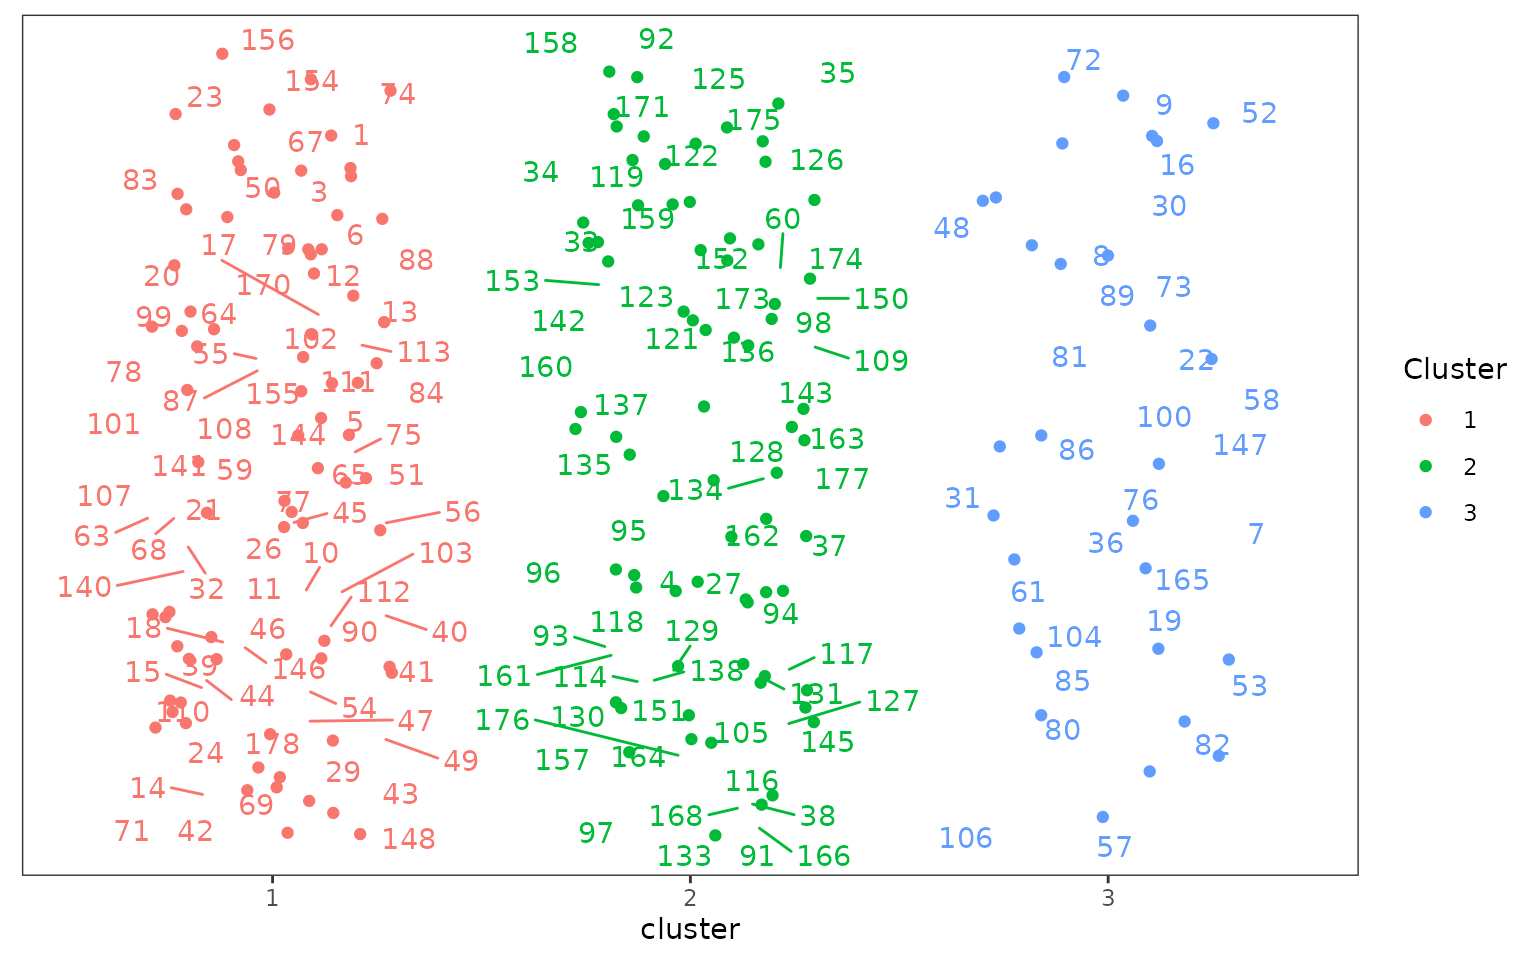
\includegraphics{Vignette-Tetrapod_files-_2_EvolRates-Selection_files/figure-latex/unnamed-chunk-6-1.pdf}

\begin{Shaded}
\begin{Highlighting}[]
\CommentTok{\#Stacked plots with viridis color scale}
\FunctionTok{clockrate\_dens\_plot}\NormalTok{(RateTable\_Medians, }\AttributeTok{stack =} \ConstantTok{TRUE}\NormalTok{, }\AttributeTok{nrow =} \DecValTok{1}\NormalTok{, }\AttributeTok{scales =} \StringTok{"fixed"}\NormalTok{)}\SpecialCharTok{+}
\NormalTok{    ggplot2}\SpecialCharTok{::}\FunctionTok{scale\_color\_viridis\_d}\NormalTok{() }\SpecialCharTok{+}
\NormalTok{    ggplot2}\SpecialCharTok{::}\FunctionTok{scale\_fill\_viridis\_d}\NormalTok{()}
\end{Highlighting}
\end{Shaded}

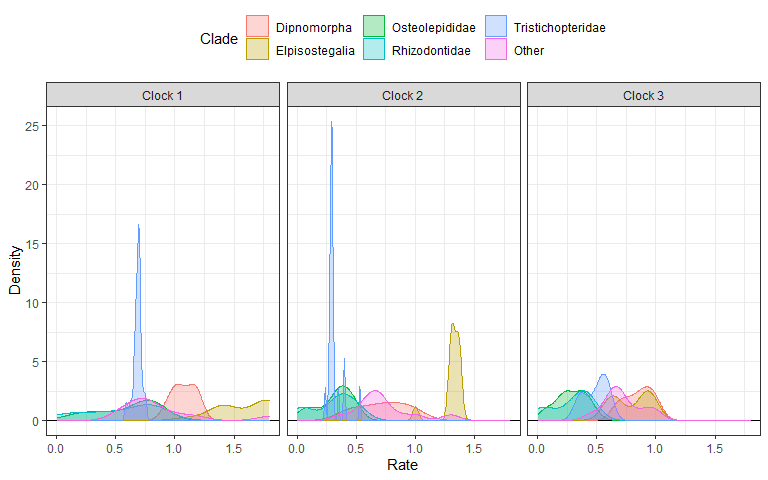
\includegraphics{Vignette-Tetrapod_files-_2_EvolRates-Selection_files/figure-latex/unnamed-chunk-7-1.pdf}

Plot linear regressions of rates from two or more clocks

\begin{Shaded}
\begin{Highlighting}[]
\CommentTok{\#Plot regressions of rates from two clocks}
\NormalTok{p12 }\OtherTok{\textless{}{-}} \FunctionTok{clockrate\_reg\_plot}\NormalTok{(RateTable\_Medians, }\AttributeTok{clock\_x =} \DecValTok{1}\NormalTok{, }\AttributeTok{clock\_y =} \DecValTok{2}\NormalTok{)}
\NormalTok{p13 }\OtherTok{\textless{}{-}} \FunctionTok{clockrate\_reg\_plot}\NormalTok{(RateTable\_Medians, }\AttributeTok{clock\_x =} \DecValTok{1}\NormalTok{, }\AttributeTok{clock\_y =} \DecValTok{3}\NormalTok{)}
\NormalTok{p23 }\OtherTok{\textless{}{-}} \FunctionTok{clockrate\_reg\_plot}\NormalTok{(RateTable\_Medians, }\AttributeTok{clock\_x =} \DecValTok{2}\NormalTok{, }\AttributeTok{clock\_y =} \DecValTok{3}\NormalTok{)}

\NormalTok{gridExtra}\SpecialCharTok{::}\FunctionTok{grid.arrange}\NormalTok{(p12, p13, p23, }\AttributeTok{nrow =} \DecValTok{2}\NormalTok{)}
\end{Highlighting}
\end{Shaded}

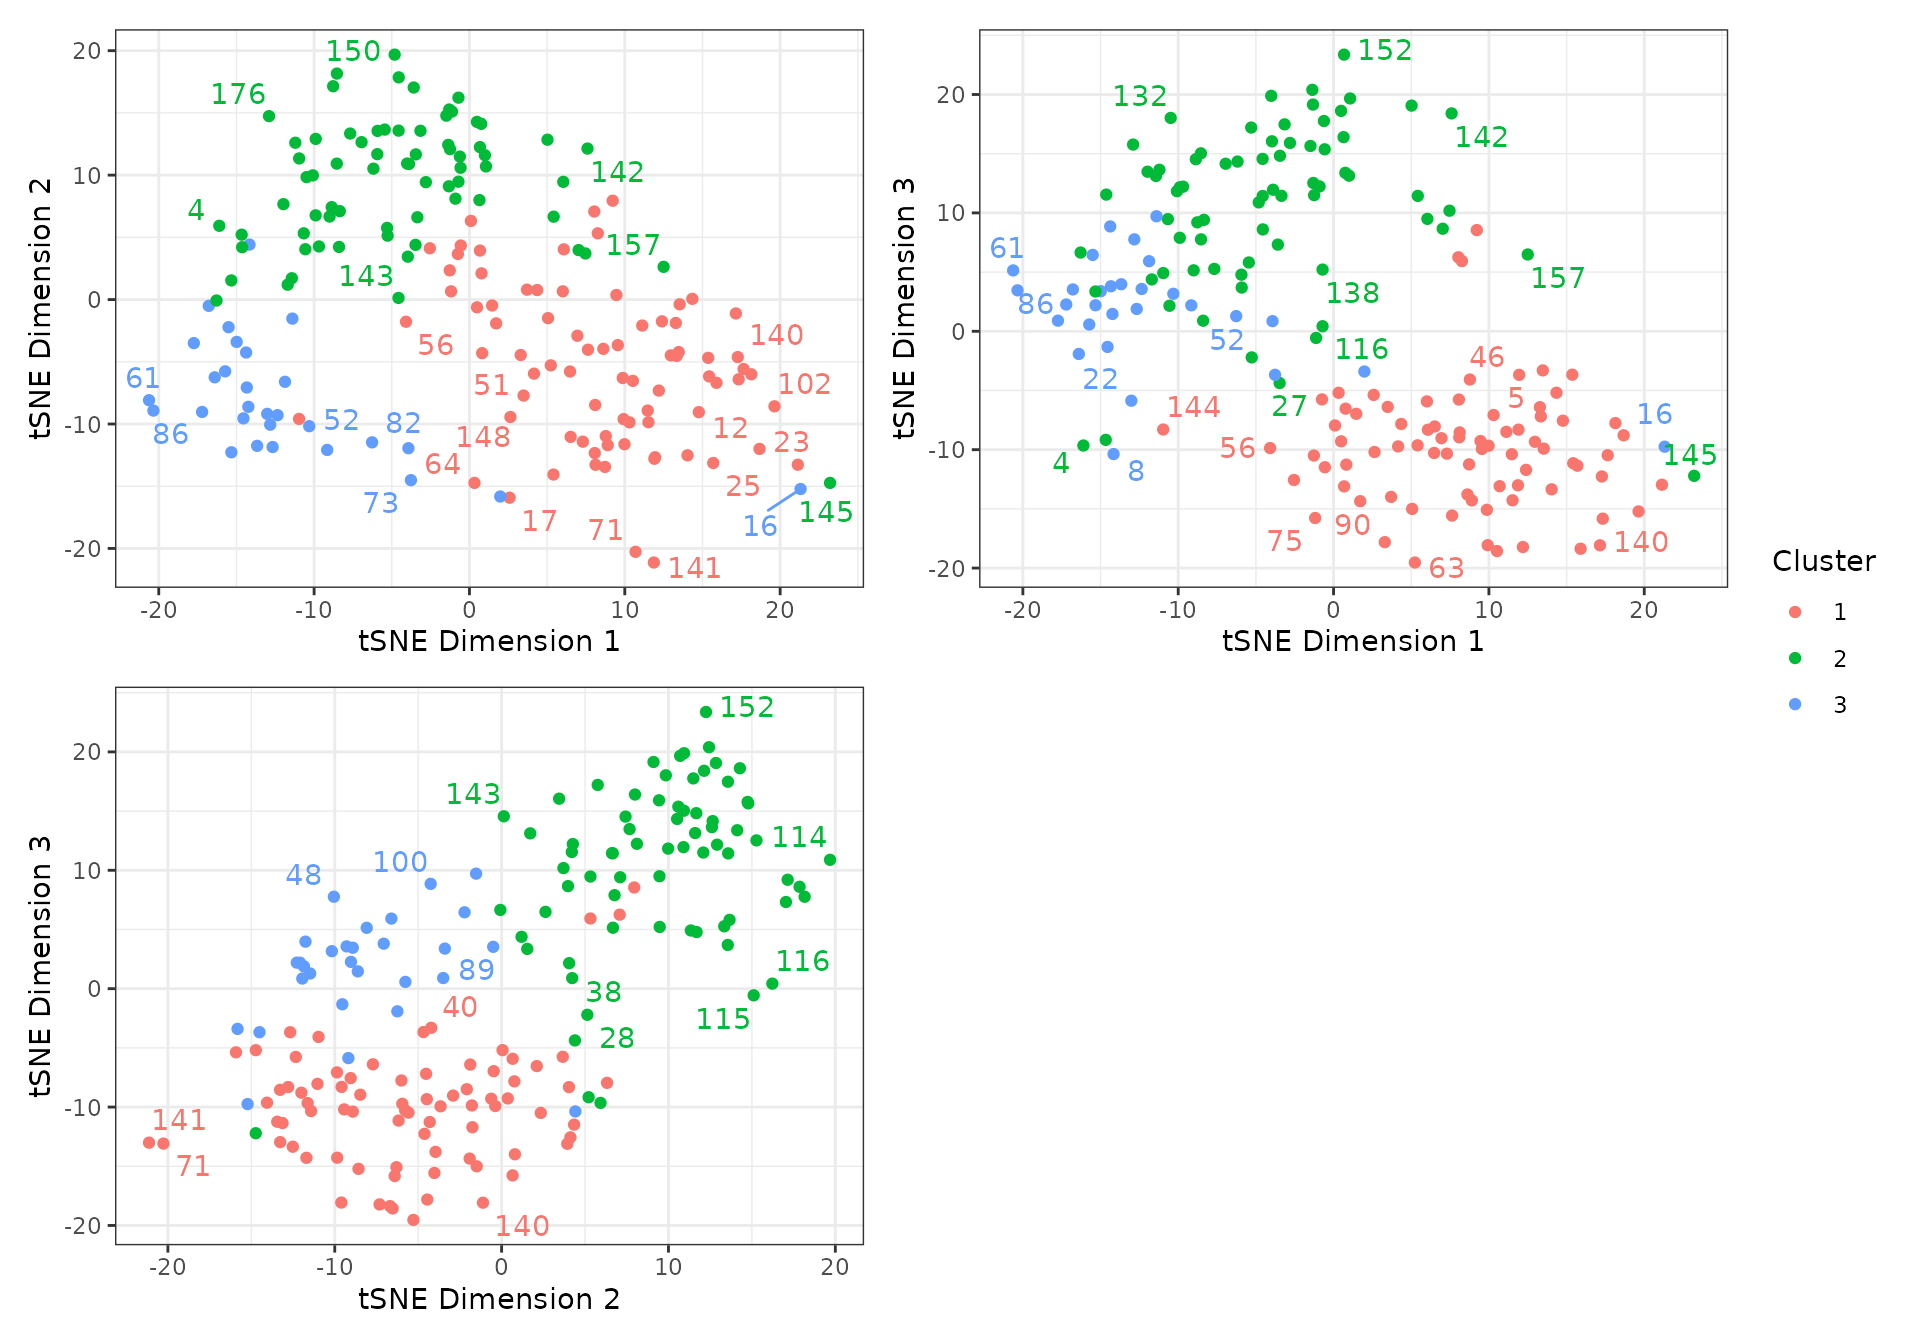
\includegraphics{Vignette-Tetrapod_files-_2_EvolRates-Selection_files/figure-latex/unnamed-chunk-8-1.pdf}

\begin{center}\rule{0.5\linewidth}{0.5pt}\end{center}

\hypertarget{selectionstrength}{%
\section{SelectionStrength}\label{selectionstrength}}

\begin{enumerate}
\def\labelenumi{\arabic{enumi}.}
\tightlist
\item
  Import rate table with customized clade membership added as an extra
  column
\end{enumerate}

\begin{Shaded}
\begin{Highlighting}[]
\CommentTok{\#Import rate table with clade membership }
\NormalTok{RateTable\_Means}\OtherTok{\textless{}{-}} \FunctionTok{read.csv}\NormalTok{(}\StringTok{"RateTable\_Means\_Clades.csv"}\NormalTok{, }\AttributeTok{header =} \ConstantTok{TRUE}\NormalTok{)}

\CommentTok{\#Transform table from wide to long format}
\NormalTok{RatesByClade }\OtherTok{\textless{}{-}} \FunctionTok{clock\_reshape}\NormalTok{(RateTable\_Means)}
\end{Highlighting}
\end{Shaded}

\begin{enumerate}
\def\labelenumi{\arabic{enumi}.}
\setcounter{enumi}{1}
\tightlist
\item
  Import combined log file from all runs. This is produced by using
  \texttt{import\_log}, or using \textbf{LogCombiner} from the
  \href{https://www.beast2.org/beagle-beast-2-in-cluster/index.html}{BEAST2}
  software package.
\end{enumerate}

\begin{Shaded}
\begin{Highlighting}[]
\CommentTok{\#Import all log (.p) files from all runs and combine them, with burn{-}in = 25\% and downsampling to 2.5k trees in each log file}
\NormalTok{Comb\_posterior3p }\OtherTok{\textless{}{-}} \FunctionTok{import\_log}\NormalTok{(}\StringTok{"E:/Git/EvoPhylo/\_dev/Examples/MultiClockTree/LogFiles3p"}\NormalTok{, }\AttributeTok{burnin =} \FloatTok{0.25}\NormalTok{, }\AttributeTok{downsample =} \DecValTok{2500}\NormalTok{)}

\CommentTok{\#OR}

\CommentTok{\#Import combined log file from all runs (if available)}
\CommentTok{\#Comb\_posterior3p \textless{}{-} read.table("3p\_CombLog(4runs).p", header = TRUE)}

\CommentTok{\#Show first 10 lines of combined log file}
\FunctionTok{head}\NormalTok{(Comb\_posterior3p, }\DecValTok{10}\NormalTok{)}
\end{Highlighting}
\end{Shaded}

\begin{verbatim}
##          Gen       LnL      LnPr  TH.all.   TL.all. prop_ancfossil.all.
## 1.1  8750000 -1449.425 -143.1907 5.271118 11.969460                   0
## 2.1  8792000 -1461.906 -132.1172 5.095504 11.083810                   0
## 3.1  8834000 -1454.645 -189.6113 3.990879  9.296558                   0
## 4.1  8876000 -1452.992 -146.6165 6.000608 13.711570                   0
## 5.1  8918000 -1439.524 -172.4858 3.970764  9.686631                   0
## 6.1  8960000 -1451.865 -123.9491 3.524645  8.246421                   0
## 7.1  9002000 -1442.711 -175.9254 5.192212 12.121940                   0
## 8.1  9044000 -1458.845 -158.1911 4.314870  9.435324                   0
## 9.1  9086000 -1459.950 -172.5915 4.801849 10.904420                   0
## 10.1 9128000 -1449.782 -201.5946 4.750418 10.530180                   0
##        sigma.1.  sigma.2.   sigma.3.      m.1.     m.2.      m.3. tk02var.1.
## 1.1  0.07660715 1.3335150 0.85234530 0.3695799 1.544579 1.3623320  0.3197728
## 2.1  0.14143120 0.5274534 1.39284900 0.4993570 1.368074 1.4454100  0.2115789
## 3.1  0.32086700 1.5483130 0.11789880 0.3728998 1.494295 1.4765140  0.5084504
## 4.1  0.28084370 1.7307190 0.27879200 0.3071567 1.667035 1.2304240  0.3488486
## 5.1  1.39133100 0.4700035 1.70377200 0.4342082 1.631227 0.9763670  0.3735620
## 6.1  0.40528960 0.4675897 0.09182396 0.4903534 1.383956 1.4307430  0.4508500
## 7.1  0.56173060 0.6716058 0.08208257 0.3706021 1.551966 1.3414990  0.4466884
## 8.1  0.72414310 1.5813640 0.20894480 0.4315873 1.600427 1.0588220  0.3127017
## 9.1  0.26363330 0.4721888 0.09480181 0.3574479 1.625353 1.1972060  0.3633493
## 10.1 0.61061390 0.3921187 0.05233850 0.3329787 1.748788 0.9608169  0.5025799
##      tk02var.2. tk02var.3. clockrate.all. Time_bin net_speciation
## 1.1   0.3848931  0.2075079    0.011927150        1     0.04987983
## 2.1   0.2723863  0.3463915    0.011605140        1     0.04990040
## 3.1   0.3962337  0.3609296    0.009110532        1     0.03255822
## 4.1   0.2993601  0.2427788    0.013514990        1     0.02019323
## 5.1   0.2696324  0.2885385    0.008887241        1     0.03916357
## 6.1   0.2565565  0.2526409    0.007887552        1     0.04679621
## 7.1   0.3683303  0.4206275    0.011692310        1     0.03205856
## 8.1   0.2879125  0.3738355    0.009753287        1     0.02404027
## 9.1   0.4158532  0.4908815    0.010940080        1     0.02908808
## 10.1  0.4800133  0.3802874    0.010758570        1     0.06569479
##      relative_extinction relative_fossilization
## 1.1            0.6785586            0.055629950
## 2.1            0.7887825            0.036796000
## 3.1            0.7515792            0.104437400
## 4.1            0.9808528            0.001310744
## 5.1            0.7422518            0.054370720
## 6.1            0.6707417            0.034095270
## 7.1            0.5995981            0.118691500
## 8.1            0.9580329            0.004336047
## 9.1            0.9204372            0.012845100
## 10.1           0.7340445            0.020493760
\end{verbatim}

\begin{enumerate}
\def\labelenumi{\arabic{enumi}.}
\setcounter{enumi}{2}
\tightlist
\item
  Produce a table of pairwise t-tests for difference between the mean
  clockrate value in the posterior and the absolute rate for each tree
  node
\end{enumerate}

\begin{Shaded}
\begin{Highlighting}[]
\CommentTok{\#Get table of pairwise t{-}tests for difference between the posterior mean and the rate for each tree node}
\NormalTok{RateSign\_tests}\OtherTok{\textless{}{-}} \FunctionTok{get\_pwt\_rates}\NormalTok{(RateTable\_Means, Comb\_posterior3p)}

\CommentTok{\#Show first 10 lines of table}
\FunctionTok{head}\NormalTok{(RateSign\_tests, }\DecValTok{10}\NormalTok{)}
\end{Highlighting}
\end{Shaded}

\begin{verbatim}
##             clade nodes clock relative rate absolute rate (mean)        null
## 1     Dipnomorpha     1     1      0.943696          0.011851072 0.011851072
## 2     Dipnomorpha     2     1      1.065326          0.013378520 0.013378520
## 3     Dipnomorpha     3     1      1.182460          0.014849506 0.014849506
## 4     Dipnomorpha     4     1      1.229767          0.015443594 0.015443594
## 5     Dipnomorpha     5     1      1.230564          0.015453603 0.015453603
## 6           Other     6     1      0.658855          0.008273997 0.008273997
## 7           Other     7     1      0.603090          0.007573692 0.007573692
## 8  Osteolepididae     8     1      0.843373          0.010591201 0.010591201
## 9  Osteolepididae     9     1      0.872012          0.010950854 0.010950854
## 10 Osteolepididae    10     1      0.811473          0.010190597 0.010190597
##          p.value
## 1  1.077126e-104
## 2  3.776689e-139
## 3   0.000000e+00
## 4   0.000000e+00
## 5   0.000000e+00
## 6   0.000000e+00
## 7   0.000000e+00
## 8   0.000000e+00
## 9   0.000000e+00
## 10  0.000000e+00
\end{verbatim}

\begin{Shaded}
\begin{Highlighting}[]
\CommentTok{\#Export the table}
\CommentTok{\#write.csv(RateSign\_tests, file="RateSign\_tests.csv")}
\end{Highlighting}
\end{Shaded}

\begin{enumerate}
\def\labelenumi{\arabic{enumi}.}
\setcounter{enumi}{3}
\tightlist
\item
  Plot selection gradient on the summary tree
\end{enumerate}

\begin{Shaded}
\begin{Highlighting}[]
\CommentTok{\#Plot tree using various thresholds}
\FunctionTok{plot\_treerates\_sgn}\NormalTok{(tree, Comb\_posterior3p, }
                   \AttributeTok{clock =} \DecValTok{1}\NormalTok{,               }\CommentTok{\#Show rates for clock partition 1}
                   \AttributeTok{summary =} \StringTok{"mean"}\NormalTok{,        }\CommentTok{\#sets summary stats to get from summary tree nodes}
                   \AttributeTok{branch\_size =} \FloatTok{1.5}\NormalTok{, }\AttributeTok{tip\_size =} \DecValTok{2}\NormalTok{,                      }\CommentTok{\#sets size for tree elements}
                   \AttributeTok{xlim=}\FunctionTok{c}\NormalTok{(}\SpecialCharTok{{-}}\DecValTok{450}\NormalTok{,}\SpecialCharTok{{-}}\DecValTok{260}\NormalTok{), }\AttributeTok{nbreaks =} \DecValTok{8}\NormalTok{, }\AttributeTok{geo\_size=}\FunctionTok{list}\NormalTok{(}\DecValTok{3}\NormalTok{, }\DecValTok{3}\NormalTok{),  }\CommentTok{\#sets limits and breaks for geoscale}
                   \AttributeTok{threshold =} \FunctionTok{c}\NormalTok{(}\StringTok{"1 SD"}\NormalTok{, }\StringTok{"2 SD"}\NormalTok{, }\StringTok{"95\%"}\NormalTok{))                 }\CommentTok{\#sets threshold for selection mode}
\end{Highlighting}
\end{Shaded}

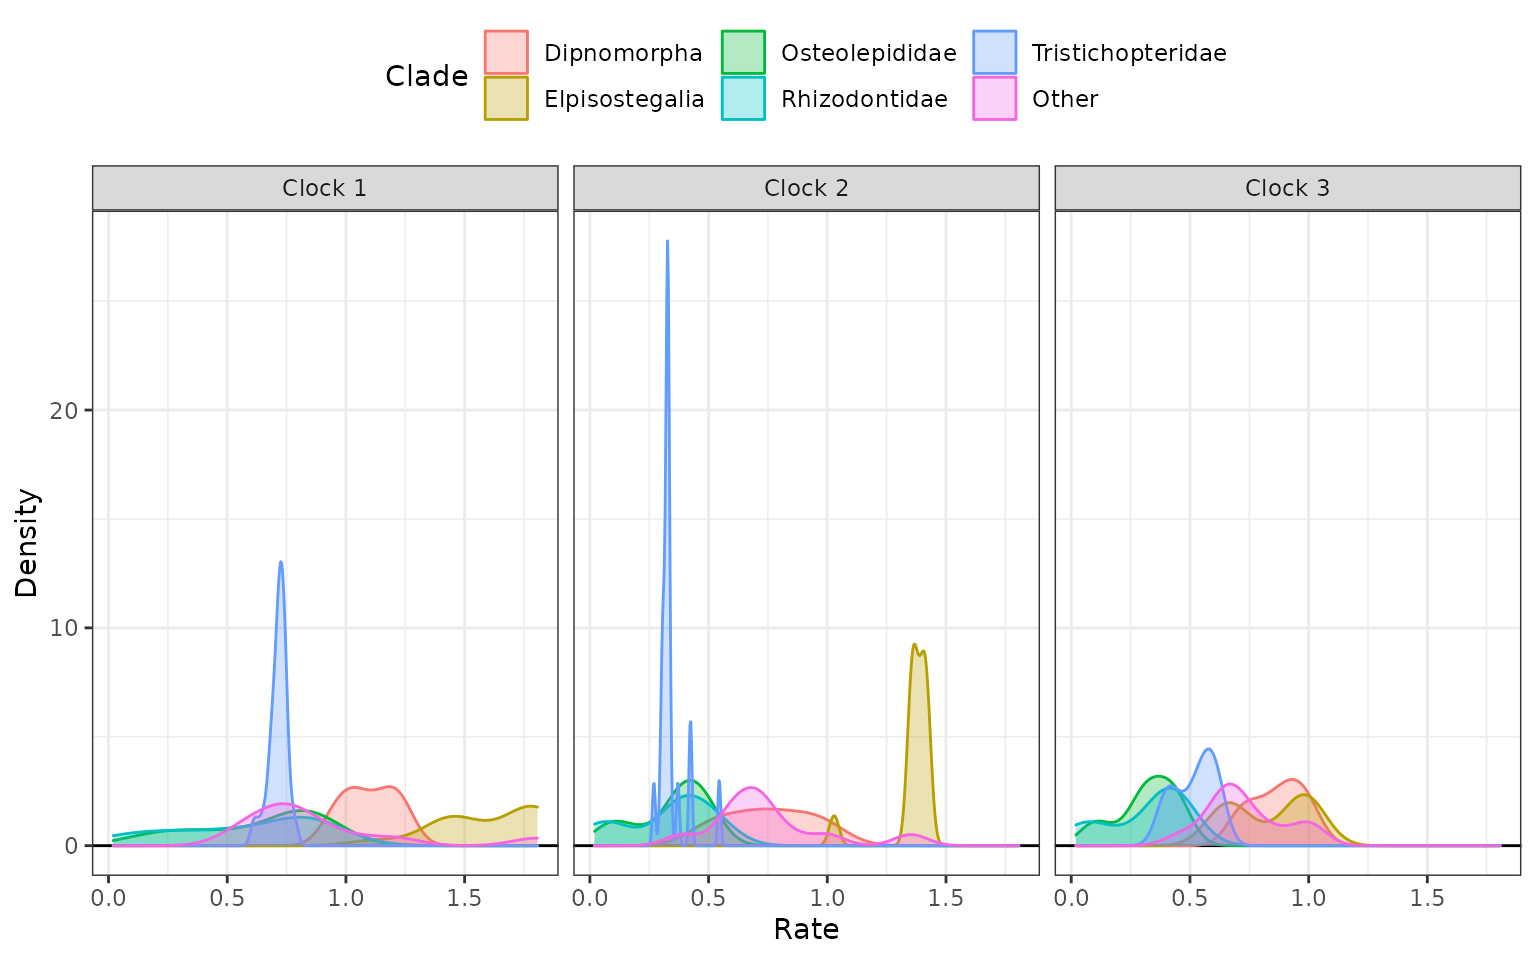
\includegraphics{Vignette-Tetrapod_files-_2_EvolRates-Selection_files/figure-latex/unnamed-chunk-12-1.pdf}

\end{document}
